\documentclass[aspectratio=43]{beamer}

% Text packages to stop warnings
\usepackage{lmodern}
\usepackage{textcomp}
\usepackage{listings}
\usepackage{multirow}
\usepackage{tikz}

\usetikzlibrary{arrows,automata,shapes,positioning}
\tikzstyle{block} = [rectangle, draw, fill=blue!20, 
    text width=2.5em, text centered, rounded corners, minimum height=2em]
\tikzstyle{bw} = [rectangle, draw, fill=blue!20, 
    text width=3.5em, text centered, rounded corners, minimum height=2em]

% Themes
\usetheme{Boadilla}
\setbeamertemplate{footline}[page number]{}
\setbeamertemplate{navigation symbols}{}

% Suppress the navigation bar
\beamertemplatenavigationsymbolsempty

\lstset{basicstyle=\scriptsize, frame=single}

\newenvironment{changemargin}[1]{% 
  \begin{list}{}{% 
    \setlength{\topsep}{0pt}% 
    \setlength{\leftmargin}{#1}% 
    \setlength{\rightmargin}{1em}
    \setlength{\listparindent}{\parindent}% 
    \setlength{\itemindent}{\parindent}% 
    \setlength{\parsep}{\parskip}% 
  }% 
  \item[]}{\end{list}} 

\title{Lecture 12---Loop-carried Dependencies; Speculation; Parallelization Patterns}
\subtitle{ECE 459: Programming for Performance}
\date{January 30, 2015}

\begin{document}

%%%%%%%%%%%%%%%%%%%%%%%%%%%%%%%%%%%%%%%%%%%%%%%%%%%%%%%%%%%%%%%%%%%%%%%%%%%%%%%%
\begin{frame}[plain]
  \titlepage
\end{frame}
%%%%%%%%%%%%%%%%%%%%%%%%%%%%%%%%%%%%%%%%%%%%%%%%%%%%%%%%%%%%%%%%%%%%%%%%%%%%%%%%

%%%%%%%%%%%%%%%%%%%%%%%%%%%%%%%%%%%%%%%%%%%%%%%%%%%%%%%%%%%%%%%%%%%%%%%%%%%%%%%%
\begin{frame}
  \frametitle{Last Time}

  \begin{changemargin}{1.5cm}
    Memory-carried dependencies:
  \end{changemargin}
\begin{center}
\begin{tabular}{ll|p{2.8cm}p{3.2cm}}
& & \multicolumn{2}{c}{Second Access} \\ 
&  & \bf Read & \bf Write \\ \hline
\multirow{2}{*}{First Access} & \bf Read & No Dependency Read After Read (RAR)  & Anti-dependency Write After Read (WAR) \\[0.5em]
& \bf Write & True Dependency Read After Write (RAW) & Output Dependency Write After Write (WAW) \\
\end{tabular}
\end{center}
  \begin{changemargin}{1.5cm}
     ~\\
    We also saw how to break WAR and WAW dependencies.\\[1em]
    Plus, loop dependencies, and Mandelbrot example.
  \end{changemargin}
\end{frame}
%%%%%%%%%%%%%%%%%%%%%%%%%%%%%%%%%%%%%%%%%%%%%%%%%%%%%%%%%%%%%%%%%%%%%%%%%%%%%%%%

\begin{frame}[fragile]
  \frametitle{Live Coding Demo: Parallelizing Mandelbrot}

  \begin{changemargin}{1.5cm}
    Refactor the code; create array for output.\\[1em]
    Add a struct to pass offset, stride to thread.\\[1em]
    Create \& join threads.
  \end{changemargin}

\end{frame}

%%%%%%%%%%%%%%%%%%%%%%%%%%%%%%%%%%%%%%%%%%%%%%%%%%%%%%%%%%%%%%%%%%%%%%%%%%%%%%%%

\part{Breaking Dependencies with Speculation}
\frame{\partpage}

%%%%%%%%%%%%%%%%%%%%%%%%%%%%%%%%%%%%%%%%%%%%%%%%%%%%%%%%%%%%%%%%%%%%%%%%%%%%%%%%
\begin{frame}
  \frametitle{Breaking Dependencies}

  \begin{changemargin}{2cm}
  \structure{Speculation}: architects use it to predict
      branch targets.
  \begin{itemize}
    \item Need not wait for the branch to be evaluated.
  \end{itemize}~\\[1em]
  We'll use speculation at a coarser-grained level:
      speculatively parallelize source code.\\[1em]

      Two ways: \structure{speculative execution} and
      \structure{value speculation}.
  \end{changemargin}
\end{frame}
%%%%%%%%%%%%%%%%%%%%%%%%%%%%%%%%%%%%%%%%%%%%%%%%%%%%%%%%%%%%%%%%%%%%%%%%%%%%%%%%


\section{Speculation}
%%%%%%%%%%%%%%%%%%%%%%%%%%%%%%%%%%%%%%%%%%%%%%%%%%%%%%%%%%%%%%%%%%%%%%%%%%%%%%%%
\begin{frame}[fragile]
  \frametitle{Speculative Execution: Example}

  \begin{changemargin}{2cm}
Consider the following code:
  
  \begin{lstlisting}
void doWork(int x, int y) {
    int value = longCalculation(x, y);
    if (value > threshold) {
      return value + secondLongCalculation(x, y);
    }
    else {
      return value;
    }
}
  \end{lstlisting}

  Will we need to run {\tt secondLongCalculation}?
  \vfill  
  \begin{itemize}
    \item<2> OK, so: could we execute {\tt longCalculation} and {\tt secondLongCalculation}
      in parallel if we didn't have the conditional?
  \end{itemize}
  \end{changemargin}
\end{frame}
%%%%%%%%%%%%%%%%%%%%%%%%%%%%%%%%%%%%%%%%%%%%%%%%%%%%%%%%%%%%%%%%%%%%%%%%%%%%%%%%

%%%%%%%%%%%%%%%%%%%%%%%%%%%%%%%%%%%%%%%%%%%%%%%%%%%%%%%%%%%%%%%%%%%%%%%%%%%%%%%%
\begin{frame}[fragile]
  \frametitle{Speculative Execution: Assume No Conditional}

  \begin{changemargin}{1.5cm}
  Yes, we could parallelize them. Consider this code:
    
    \begin{lstlisting}
  void doWork(int x, int y) {
    thread_t t1, t2;
    point p(x,y);
    int v1, v2;
    thread_create(&t1, NULL, &longCalculation, &p);
    thread_create(&t2, NULL, &secondLongCalculation, &p);
    thread_join(t1, &v1);
    thread_join(t2, &v2);
    if (v1 > threshold) {
      return v1 + v2;
    } else {
      return v1;
    }
  }
    \end{lstlisting}

  We do both the calculations in parallel and return the same result as before.

  \begin{itemize}
    \item What are we assuming about {\tt longCalculation} and
{\tt secondLongCalculation}?
  \end{itemize}
  \end{changemargin}
\end{frame}
%%%%%%%%%%%%%%%%%%%%%%%%%%%%%%%%%%%%%%%%%%%%%%%%%%%%%%%%%%%%%%%%%%%%%%%%%%%%%%%%

%%%%%%%%%%%%%%%%%%%%%%%%%%%%%%%%%%%%%%%%%%%%%%%%%%%%%%%%%%%%%%%%%%%%%%%%%%%%%%%%
\begin{frame}
  \frametitle{Estimating Impact of Speculative Execution}

  \begin{changemargin}{2.5cm}
  $T_1$: time to run {\tt longCalculatuion}.

  $T_2$: time to run {\tt secondLongCalculation}.

  $p$: probability that {\tt secondLongCalculation} executes.\\[1em]

  In the normal case we have:
    \[T_{\mbox{\scriptsize normal}} = T_1 + pT_2.\]

  $S$: synchronization overhead.\\
  Our speculative code takes:
    \[ T_{\mbox{\scriptsize speculative}} = \mbox{max}(T_1, T_2) + S.\]

    \structure{Exercise.} When is speculative code faster? Slower? \\ How could you improve it?

  \end{changemargin}
\end{frame}
%%%%%%%%%%%%%%%%%%%%%%%%%%%%%%%%%%%%%%%%%%%%%%%%%%%%%%%%%%%%%%%%%%%%%%%%%%%%%%%%

%%%%%%%%%%%%%%%%%%%%%%%%%%%%%%%%%%%%%%%%%%%%%%%%%%%%%%%%%%%%%%%%%%%%%%%%%%%%%%%%
\begin{frame}[fragile]
  \frametitle{Shortcomings of Speculative Execution}

  \begin{changemargin}{2cm}
  Consider the following code:
  
  \begin{lstlisting}
void doWork(int x, int y) {
    int value = longCalculation(x, y);
    return secondLongCalculation(value);
}
  \end{lstlisting}

  Now we have a true dependency; can't use speculative~execution.\\[1em]

  But: if the value is predictable, we can execute
      {\tt secondLongCalculation} using the predicted value.\\[1em]

  This is \structure{value speculation}.
  \end{changemargin}
\end{frame}
%%%%%%%%%%%%%%%%%%%%%%%%%%%%%%%%%%%%%%%%%%%%%%%%%%%%%%%%%%%%%%%%%%%%%%%%%%%%%%%%

%%%%%%%%%%%%%%%%%%%%%%%%%%%%%%%%%%%%%%%%%%%%%%%%%%%%%%%%%%%%%%%%%%%%%%%%%%%%%%%%
\begin{frame}[fragile]
  \frametitle{Value Speculation Implementation}

% note: v1 is meant to be the result you get from longCalculation this time, while last_value is what you got last time. (The code doesn't show that). If you get the same result from longCalculation this time as you did last time, then secondLongCalculation is correct and you don't need to redo it.
  \begin{changemargin}{2cm}
  This Pthread code does value speculation:
  
  \begin{lstlisting}
void doWork(int x, int y) {
    thread_t t1, t2;
    point p(x,y);
    int v1, v2, last_value;
    thread_create(&t1, NULL, &longCalculation, &p);
    thread_create(&t2, NULL, &secondLongCalculation,
                  &last_value);
    thread_join(t1, &v1);
    thread_join(t2, &v2);
    if (v1 == last_value) {
      return v2;
    } else {
      last_value = v1;
      return secondLongCalculation(v1);
    }
}
  \end{lstlisting}

  Note: this is like memoization (plus parallelization).
  \end{changemargin}
\end{frame}
%%%%%%%%%%%%%%%%%%%%%%%%%%%%%%%%%%%%%%%%%%%%%%%%%%%%%%%%%%%%%%%%%%%%%%%%%%%%%%%%

%%%%%%%%%%%%%%%%%%%%%%%%%%%%%%%%%%%%%%%%%%%%%%%%%%%%%%%%%%%%%%%%%%%%%%%%%%%%%%%%
\begin{frame}
  \frametitle{Estimating Impact of Value Speculation}

  \begin{changemargin}{2.5cm}
  $T_1$: time to run {\tt longCalculatuion}.

  $T_2$: time to run {\tt secondLongCalculation}.

  $p$: probability that {\tt secondLongCalculation} executes.

  $S$: synchronization overhead.\\[1em]

  In the normal case, we again have:
    \[ T = T_1 +pT_2.\]

  This speculative code takes:
    \[ T = \mbox{max}(T_1, T_2) + S + pT_2.\]

    \structure{Exercise.} Again, when is speculative code faster? Slower? How could you improve it?

  \end{changemargin}
\end{frame}
%%%%%%%%%%%%%%%%%%%%%%%%%%%%%%%%%%%%%%%%%%%%%%%%%%%%%%%%%%%%%%%%%%%%%%%%%%%%%%%%

%%%%%%%%%%%%%%%%%%%%%%%%%%%%%%%%%%%%%%%%%%%%%%%%%%%%%%%%%%%%%%%%%%%%%%%%%%%%%%%%
\begin{frame}
  \frametitle{When Can We Speculate?}

  \begin{changemargin}{2.5cm}
  Required conditions for safety:

  \begin{itemize}
    \item {\tt longCalculation} and {\tt secondLongCalculation} must not call
      each other.
    \item {\tt secondLongCalculation} must not depend on
      any values set or modified by {\tt longCalculation}.
    \item The return value of {\tt longCalculation} must be deterministic.
  \end{itemize}

  General warning: Consider \structure{side effects} of function calls.
  \end{changemargin}
\end{frame}
%%%%%%%%%%%%%%%%%%%%%%%%%%%%%%%%%%%%%%%%%%%%%%%%%%%%%%%%%%%%%%%%%%%%%%%%%%%%%%%%

  \part{Parallelization Patterns}
\frame{\partpage}

%%%%%%%%%%%%%%%%%%%%%%%%%%%%%%%%%%%%%%%%%%%%%%%%%%%%%%%%%%%%%%%%%%%%%%%%%%%%%%%%
\begin{frame}
  \frametitle{Critical Paths}

  \begin{changemargin}{2.5cm}

  Should be familiar with critcal paths from other courses (Gantt charts).\\[1em]

  Consider the following diagram (edges are tasks):

\begin{center}
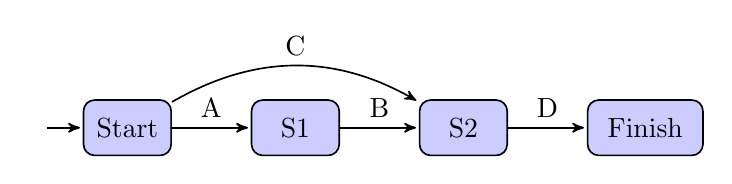
\begin{tikzpicture}[->,>=stealth',shorten >=1pt,auto,column sep=2.2cm,
                    semithick,initial text=]
  \node[initial,block] (s0) {Start};
  \node[block] (s1) [right=of s0] {S1};
  \node[block] (s2) [right=of s1] {S2};
  \node[bw] (s3) [right=of s2] {Finish};

  \path (s0) edge node {A} (s1)
        (s1) edge node {B} (s2)
        (s2) edge node {D} (s3)
        (s0) edge[bend left=30] node {C} (s2);
\end{tikzpicture}
\end{center}

  \begin{itemize}
    \item B depends on A, C has no dependencies, and D depends on B and C.
    \item Can execute A-then-B in parallel with C.
    \item Keep dependencies in mind when calculating speedups for more
      complex programs.
  \end{itemize}
  \end{changemargin}
\end{frame}
%%%%%%%%%%%%%%%%%%%%%%%%%%%%%%%%%%%%%%%%%%%%%%%%%%%%%%%%%%%%%%%%%%%%%%%%%%%%%%%%

%%%%%%%%%%%%%%%%%%%%%%%%%%%%%%%%%%%%%%%%%%%%%%%%%%%%%%%%%%%%%%%%%%%%%%%%%%%%%%%%
\begin{frame}
  \frametitle{Data and Task Parallelism}

  \begin{changemargin}{2.5cm}
     \structure{Data parallelism} is performing \emph{the same} operations on
      different input.\\

     {\bf Example:} doubling all elements of an array.\\[1em]

     \structure{Task parallelism} is performing \emph{different} operations
      on different input.

    {\bf Example:} playing a video file: one thread decompresses
      frames, another renders.

  \end{changemargin}
\end{frame}
%%%%%%%%%%%%%%%%%%%%%%%%%%%%%%%%%%%%%%%%%%%%%%%%%%%%%%%%%%%%%%%%%%%%%%%%%%%%%%%%

%%%%%%%%%%%%%%%%%%%%%%%%%%%%%%%%%%%%%%%%%%%%%%%%%%%%%%%%%%%%%%%%%%%%%%%%%%%%%%%%
\begin{frame}
  \frametitle{Data Parallelism: Single Instruction, Multiple Data}

  \begin{changemargin}{2cm}
    We'll discuss SIMD in more detail later. An overview:
    \begin{itemize}
    \item You can load a bunch of data and perform 
      arithmetic.
    \item Intructions process multiple data items simultaneously.
      (Exact number is hardware-dependent).
    \end{itemize}
    For x86-class CPUs, MMX and SSE extensions provide SIMD instructions.
  \end{changemargin}
\end{frame}
%%%%%%%%%%%%%%%%%%%%%%%%%%%%%%%%%%%%%%%%%%%%%%%%%%%%%%%%%%%%%%%%%%%%%%%%%%%%%%%%

%%%%%%%%%%%%%%%%%%%%%%%%%%%%%%%%%%%%%%%%%%%%%%%%%%%%%%%%%%%%%%%%%%%%%%%%%%%%%%%%
\begin{frame}[fragile]
  \frametitle{SIMD Example}

  \begin{changemargin}{1.5cm}
  Consider the following code:

  \begin{lstlisting}
void vadd(double * restrict a, double * restrict b, 
          int count) {
  for (int i = 0; i < count; i++)
    a[i] += b[i];
}    
  \end{lstlisting}

    In this scenario, we have a regular operation over block data.\\[1em]

    We could use threads, but we'll use SIMD.

  \end{changemargin}
\end{frame}
%%%%%%%%%%%%%%%%%%%%%%%%%%%%%%%%%%%%%%%%%%%%%%%%%%%%%%%%%%%%%%%%%%%%%%%%%%%%%%%%

%%%%%%%%%%%%%%%%%%%%%%%%%%%%%%%%%%%%%%%%%%%%%%%%%%%%%%%%%%%%%%%%%%%%%%%%%%%%%%%%
\begin{frame}[fragile]
  \frametitle{SIMD Example---Assembly without SIMD}

  \begin{changemargin}{1.5cm}
If we compile this without SIMD instructions on a 32-bit x86, (flags {\tt -m32 -march=i386 -S}) we might get this:

  \begin{lstlisting}
loop:
  fldl  (%edx)
  faddl (%ecx)
  fstpl (%edx)
  addl  8, %edx
  addl  8, %ecx
  addl  1, %esi
  cmp   %eax, %esi
  jle   loop
  \end{lstlisting}

   Just loads, adds, writes and increments.
  \end{changemargin}
\end{frame}
%%%%%%%%%%%%%%%%%%%%%%%%%%%%%%%%%%%%%%%%%%%%%%%%%%%%%%%%%%%%%%%%%%%%%%%%%%%%%%%%


%%%%%%%%%%%%%%%%%%%%%%%%%%%%%%%%%%%%%%%%%%%%%%%%%%%%%%%%%%%%%%%%%%%%%%%%%%%%%%%%
\begin{frame}[fragile]
  \frametitle{SIMD Example---Assembly with SIMD}

  \begin{changemargin}{1.5cm}
 Instead, compiling to SIMD instructions\\ ({\tt -m32 -mfpmath=sse -march=prescott}) gives:

  \begin{lstlisting}
loop:
  movupd (%edx),%xmm0
  movupd (%ecx),%xmm1
  addpd  %xmm1,%xmm0
  movpd  %xmm0,(%edx)
  addl   16,%edx
  addl   16,%ecx
  addl   2,%esi
  cmp    %eax,%esi
  jle    loop
  \end{lstlisting}

  \begin{itemize}
    \item Now processing two elements at a time on the same core.
    \item Also, no need for stack-based x87 code.
  \end{itemize}
  \end{changemargin}
\end{frame}
%%%%%%%%%%%%%%%%%%%%%%%%%%%%%%%%%%%%%%%%%%%%%%%%%%%%%%%%%%%%%%%%%%%%%%%%%%%%%%%%

%%%%%%%%%%%%%%%%%%%%%%%%%%%%%%%%%%%%%%%%%%%%%%%%%%%%%%%%%%%%%%%%%%%%%%%%%%%%%%%%
\begin{frame}
  \frametitle{SIMD Overview}

  \begin{changemargin}{1cm}
  \begin{itemize}
    \item Operations \emph{packed}: operate on multiple data elements 
      at~the~same~time.
    \vfill
    \item On modern 64-bit CPUs, SSE has 16 128-bit registers.
    \vfill
    \item Very good if your data can be \emph{vectorized} and performs math.
    \vfill
    \item Usual application: image/video processing.
    \vfill
    \item We'll see more SIMD as we get into GPU programming: GPUs excel
       at these types of applications.
  \end{itemize}
  \end{changemargin}

\end{frame}
%%%%%%%%%%%%%%%%%%%%%%%%%%%%%%%%%%%%%%%%%%%%%%%%%%%%%%%%%%%%%%%%%%%%%%%%%%%%%%%%


\end{document}
